\documentclass[a4paper,twocolumn]{article}


\usepackage[sc]{mathpazo} % Use the Palatino font
\usepackage[T1]{fontenc} % Use 8-bit encoding that has 256 glyphs
\usepackage[utf8]{inputenc} % Use utf-8 as encoding
\linespread{1.05} % Line spacing - Palatino needs more space between lines
\usepackage{microtype} % Slightly tweak font spacing for aesthetics
\usepackage{graphicx}

\usepackage[spanish]{babel} % Language hyphenation and typographical rules
%\usepackage[galician]{babel} % Change to this if using galician

\usepackage[hmarginratio=1:1,top=32mm,columnsep=20pt]{geometry} % Document margins
\usepackage[hang, small,labelfont=bf,up,textfont=it,up]{caption} % Custom captions under/above floats in tables or figures
\usepackage{booktabs} % Horizontal rules in tables

\usepackage{enumitem} % Customized lists
\setlist[itemize]{noitemsep} % Make itemize lists more compact

\usepackage{abstract} % Allows abstract customization
\renewcommand{\abstractnamefont}{\normalfont\bfseries} % Set the "Abstract" text to bold
\renewcommand{\abstracttextfont}{\normalfont\small\itshape} % Set the abstract itself to small italic text

\usepackage{titlesec} % Allows customization of titles
\renewcommand\thesection{\Roman{section}} % Roman numerals for the sections
\renewcommand\thesubsection{\Alph{subsection}} % roman numerals for subsections
\titleformat{\section}[block]{\large\scshape\centering}{\thesection.}{1em}{} % Change the look of the section titles
\titleformat{\subsection}[block]{\large}{\thesubsection.}{1em}{} % Change the look of the section titles

\usepackage{fancyhdr} % Headers and footers
\pagestyle{fancy} % All pages have headers and footers
\fancyhead{} % Blank out the default header
\fancyfoot{} % Blank out the default footer
%\fancyhead[C]{Running title $\bullet$ May 2016 $\bullet$ Vol. XXI, No. 1} % Custom header text
\fancyfoot[C]{\thepage} % Custom footer text

\usepackage{titling} % Customizing the title section

\usepackage{hyperref} % For hyperlinks in the PDF

\usepackage{listings}
\usepackage{xcolor}

\usepackage{float}

\usepackage{amsmath}

% Configuración de los listings para mostrar código
\lstset{
    language=C,                % Lenguaje de programación
    basicstyle=\small\ttfamily, % Estilo básico y tamaño de fuente
    keywordstyle=\color{blue}, % Estilo de las palabras clave
    stringstyle=\color{red},   % Estilo de las cadenas de texto
    commentstyle=\color{purple},% Estilo de los comentarios
    morecomment=[l][\color{magenta}]{\#},  % Estilo de los preprocesadores
    breaklines=true,           % Permite que las líneas se partan
    breakatwhitespace=true,    % Los cortes de línea ocurren en los espacios en blanco
    tabsize=4,                 % Tamaño de tabulación
    showstringspaces=false,    % No muestra espacios especiales en las cadenas
    frame=single,              % Añade un marco alrededor del código
    numbers=left,              % Números de línea a la izquierda
    numberstyle=\small,        % Tamaño de fuente de los números de línea
    captionpos=b,              % Posición del título en la parte inferior
    escapeinside={(*@}{@*)}    % Permite añadir LaTeX dentro del código
}

%----------------------------------------------------------------------------------------
%	TITLE SECTION
%----------------------------------------------------------------------------------------

\setlength{\droptitle}{-4\baselineskip} % Move the title up

\pretitle{\begin{center}\huge\bfseries} % Article title formatting
	\posttitle{\end{center}} % Article title closing formatting

\title{Desenrolle de lazos internos con optimización de operaciones de reducción} % Article title

\date{\today} % Leave empty to omit a date
\renewcommand{\maketitlehookd}{%
	\begin{abstract}
		\noindent En este informe, se abordará el tema del desenrolle de lazos para la optimización de operaciones de reducción, tal que se verá en que consiste la técnica y se comentarán experimentos.  \\\mbox{}\\
		 \textbf{\textit{Palabras clave}: bucles, lazos, unrolling, desenrollamiento, optimización\ldots}
	\end{abstract}
}

%----------------------------------------------------------------------------------------

\begin{document}
	
	% Print the title
	\maketitle
	
	%----------------------------------------------------------------------------------------
	%	ARTICLE CONTENTS
	%----------------------------------------------------------------------------------------
	
	\section{Introducción}

        En el presente informe se describe una serie de experimentos diseñados para estudiar la técnica denominada desenrollamiento de lazos, en el contexto de operaciones de reducción.
        
        Para el estudio, se realizarán varios programas breves escritos en el lenguaje de bajo nivel C, ejecutados en un sistema operativo UNIX. Para la medición de los tiempos de ejecución de los bucles for se utilizará la librería \textit{sys/time.h}.

 
%	Introducción al problema tratado, incluyendo las referencias  necesarias. Por ejemplo: ``Este trabajo se basa en los estudios teóricos realizados en~\cite{Intel:2005} y \cite{spec}". En este apartado se plantean el problema a resolver, objetivos a alcanzar y metodología seguida para alcanzarlos.
	
%	Es una introducción al problema, no se desarrollarán los contenidos aquí. 
	
%	La introducción termina indicando en pocas palabras de qué secciones consta el resto del documento y de qué trata cada una. Se mencionan todas las secciones salvo la de referencias (bibliografía). 

	%------------------------------------------------
	
%-------------------------------------------

\section{Descripción de la técnica analizada: Loop Unrolling}

El desenrollamiento de lazos (loop unrollig en inglés), es una técnica que consiste en intentar minimizar el coste temporal de un bucle o lazo, mediante la reducción del número de iteraciones del mismo. 

Básicamente lo que hacemos en esta es la de eliminar o reducir las iteraciones necesarias para realizar una operación, reduciendo así el tiempo de ejecución de la misma. 

Un sencillo ejemplo es el siguiente:

\begin{lstlisting}[caption={Bucle sin desenrollar},label={lst:codigoC}]
	// This program does not uses loop unrolling. 
	#include<stdio.h> 
	
	int main(void) 
	{ 
		for (int i=0; i<5; i++) 
			printf("Hello\n"); //print hello 5 times 
	
		return 0; 
	}
\end{lstlisting}

\begin{lstlisting}[caption={Bucle aplicando la técnica},label={lst:codigoC}]
	// This program uses loop unrolling. 
	#include<stdio.h> 
	
	int main(void) 
	{ 
		// unrolled the for loop in program 1 
		printf("Hello\n"); 
		printf("Hello\n"); 
		printf("Hello\n"); 
		printf("Hello\n"); 
		printf("Hello\n"); 
	
		return 0; 
	} 
\end{lstlisting}

Ambos programas [1] nos muestran un sencillo ejemplo de la aplicación de esta técnica, pudiendo observar en el segundo caso se ha eliminado por completo el bucle, reduciendo así el tiempo de ejecución del programa, debido a que dentro del bucle es necesario hacer una comprobación del índice, lo que ralentiza el código. 

Otra manera diferente, para lazos donde eliminar el bucle por completo no es posible, se pueden reducir el número de iteraciones realizando varias operaciones en una sola iteración. 

Por ejemplo: imaginemos que tenemos un bucle el cual almacena en una variable el sumatorio de los números del 1 al 10. En un bucle sin desenrollamiento tendríamos que realizar 10 iteraciones, donde en cada una realizamos una operación. Sin embargo, podemos reducir el número de iteraciones a la mitad si en vez de sumar de uno en uno, sumamos de dos en dos, y a su vez podríamos reducirlo a 2 iteraciones si sumamos de 5 en 5. Esto es la otra manera (y que a su vez veremos posteriormente en los experimentos) de aplicar la técnica de desenrollamiento de lazos.

\section{Beneficios y desventajas}

Como casi cualquier herramienta que podamos utilizar, esta técnica conlleva una serie de ventajas y desventajas. Algunas de las ventajas que podemos encontrar son:

\textbf{Ventajas:}
\begin{enumerate}
	\item \textbf{Reducción de la Sobrecarga de Ciclos de Bucle:} En cualquier sistema, reducir la frecuencia con la que se evalúan las condiciones del bucle y se actualizan las variables de control puede mejorar el rendimiento al disminuir la sobrecarga general del bucle.
	\item \textbf{Incremento en el Paralelismo:} En sistemas con capacidades de procesamiento paralelo, desenrollar bucles puede permitir que múltiples operaciones se ejecuten al mismo tiempo, mejorando el uso del paralelismo inherente al hardware.
	\item \textbf{Mejor Uso de las Unidades de Procesamiento:} Al desenrollar un bucle, se pueden realizar más cálculos por cada entrada al bucle, lo cual puede ser eficiente en términos de aprovechamiento del tiempo de CPU y la ejecución en pipelining.
    \item \textbf{Reducción en el Tiempo de Ciclo de Reloj:} A medida que se desenrollan los bucles y el área utilizada se reduce inicialmente, puede resultar en un decremento en el tiempo de ciclo de reloj, lo cual potencialmente incrementa la frecuencia de operación y por ende la velocidad de procesamiento.
    \item \textbf{Disminución en el Uso del Área de FPGA (Field Programmable Gate Array) en Ciertos Casos:} Inicialmente, el desenrollamiento puede llevar a una reducción en el área utilizada, lo que es beneficioso cuando el área es una limitante crítica en el diseño del sistema.
\end{enumerate}

\textbf{Desventajas:}
\begin{enumerate}
	\item \textbf{Aumento del Tamaño del Código:} Desenrollar bucles aumenta la cantidad de código que se ejecuta, lo cual puede llevar a un mayor uso de la memoria de instrucciones y potencialmente a un caché de instrucciones más ocupado.
	\item \textbf{Complicaciones en la Gestión de la Memoria:} El aumento en la cantidad de operaciones ejecutadas simultáneamente puede hacer que la gestión de memoria sea más compleja y puede presionar al ancho de banda de memoria disponible.
	\item \textbf{Limitaciones por Dependencias de Datos:} Si existen dependencias de datos dentro de las iteraciones de un bucle, el desenrollamiento puede no ser aplicable sin modificar significativamente el algoritmo o puede llevar a la ejecución ineficiente debido a la espera de datos.
	\item \textbf{Inflexibilidad en la Modificación del Código:} El código desenrollado es menos flexible para modificaciones futuras o ajustes de parámetros del bucle, ya que cualquier cambio requiere más esfuerzo para actualizar todas las instancias desenrolladas del bucle.
\end{enumerate}

Por tanto, viendo las ventajas y las desventajas, el programador deberá valorar si aplicar esta técnica en su código, ya que aunque puede mejorar el rendimiento, también puede conllevar una serie de problemas.

\section{Experimentos}

Para los experimentos, se ha realizado un programa en C que mide los dos siguiente bucles:

\begin{lstlisting}[caption={Bucle sin desenrollar},label={lst:codigoC}]
	for(k=0; k<ITER; k++){
        a=0.0;
        for(i=0; i<N; i++){
            a = a + x[i] * y[i];
        }
    }
\end{lstlisting}

\begin{lstlisting}[caption={Bucle aplicando la técnica},label={lst:codigoC}]
	for(k=0; k<ITER; k++){
        a = a1 = a2 = a3 = 0.0;

        for(i=0; i<N; i+=4){
            a = a + x[i] * y[i];
            a1 = a1 + x[i+1] * y[i+1];
            a2 = a2 + x[i+2] * y[i+2];
            a3 = a3 + x[i+3] * y[i+3];
        }   

        a = a + a1 + a2 + a3;
    } 
\end{lstlisting}

En el primer bucle [3], se realiza la operación de producto escalar de dos vectores de tamaño N, y se repite ITER veces. En el segundo bucle [4], se ha desenrollado el bucle interno, realizando 4 operaciones en cada iteración.

Por tanto sobre estos dos lazos realizarán experimentos modificando el valor de N y de ITER, para ver como afecta el desenrollamiento de lazos en el tiempo de ejecución del programa.

Un detalle a destacar sobre la implementación del código, es la necesidad de limpiar la caché antes de realizar las mediciones, ya que si no se hace, puede afectar a la precisión de los datos medidos. Para ello, se ha implementado la función \textit{clearCache()} la cual, sirviéndose del tamaño de la caché L1d, crea un array de este tamaño para posteriormente rellenarlo entero y posteriormente liberándolo. Debido al tamaño del programa no es necesario limpiar la caché L2, ya que el tamaño de la anterior es de 64KB, y no llega a sobrepasar este tamaño.

\subsection{Tiempos de ejecución}

Para el primer experimento vamos a realizar una serie de mediciones variando el tamaño de ITER, con un tamaño de array fijo, y veremos como afecta al tiempo de ejecución del programa.

Para analizarlo correctamente nos serviremos de la siguiente gráfica:

\begin{figure}[H]
    \centering
    \hspace{1cm}
    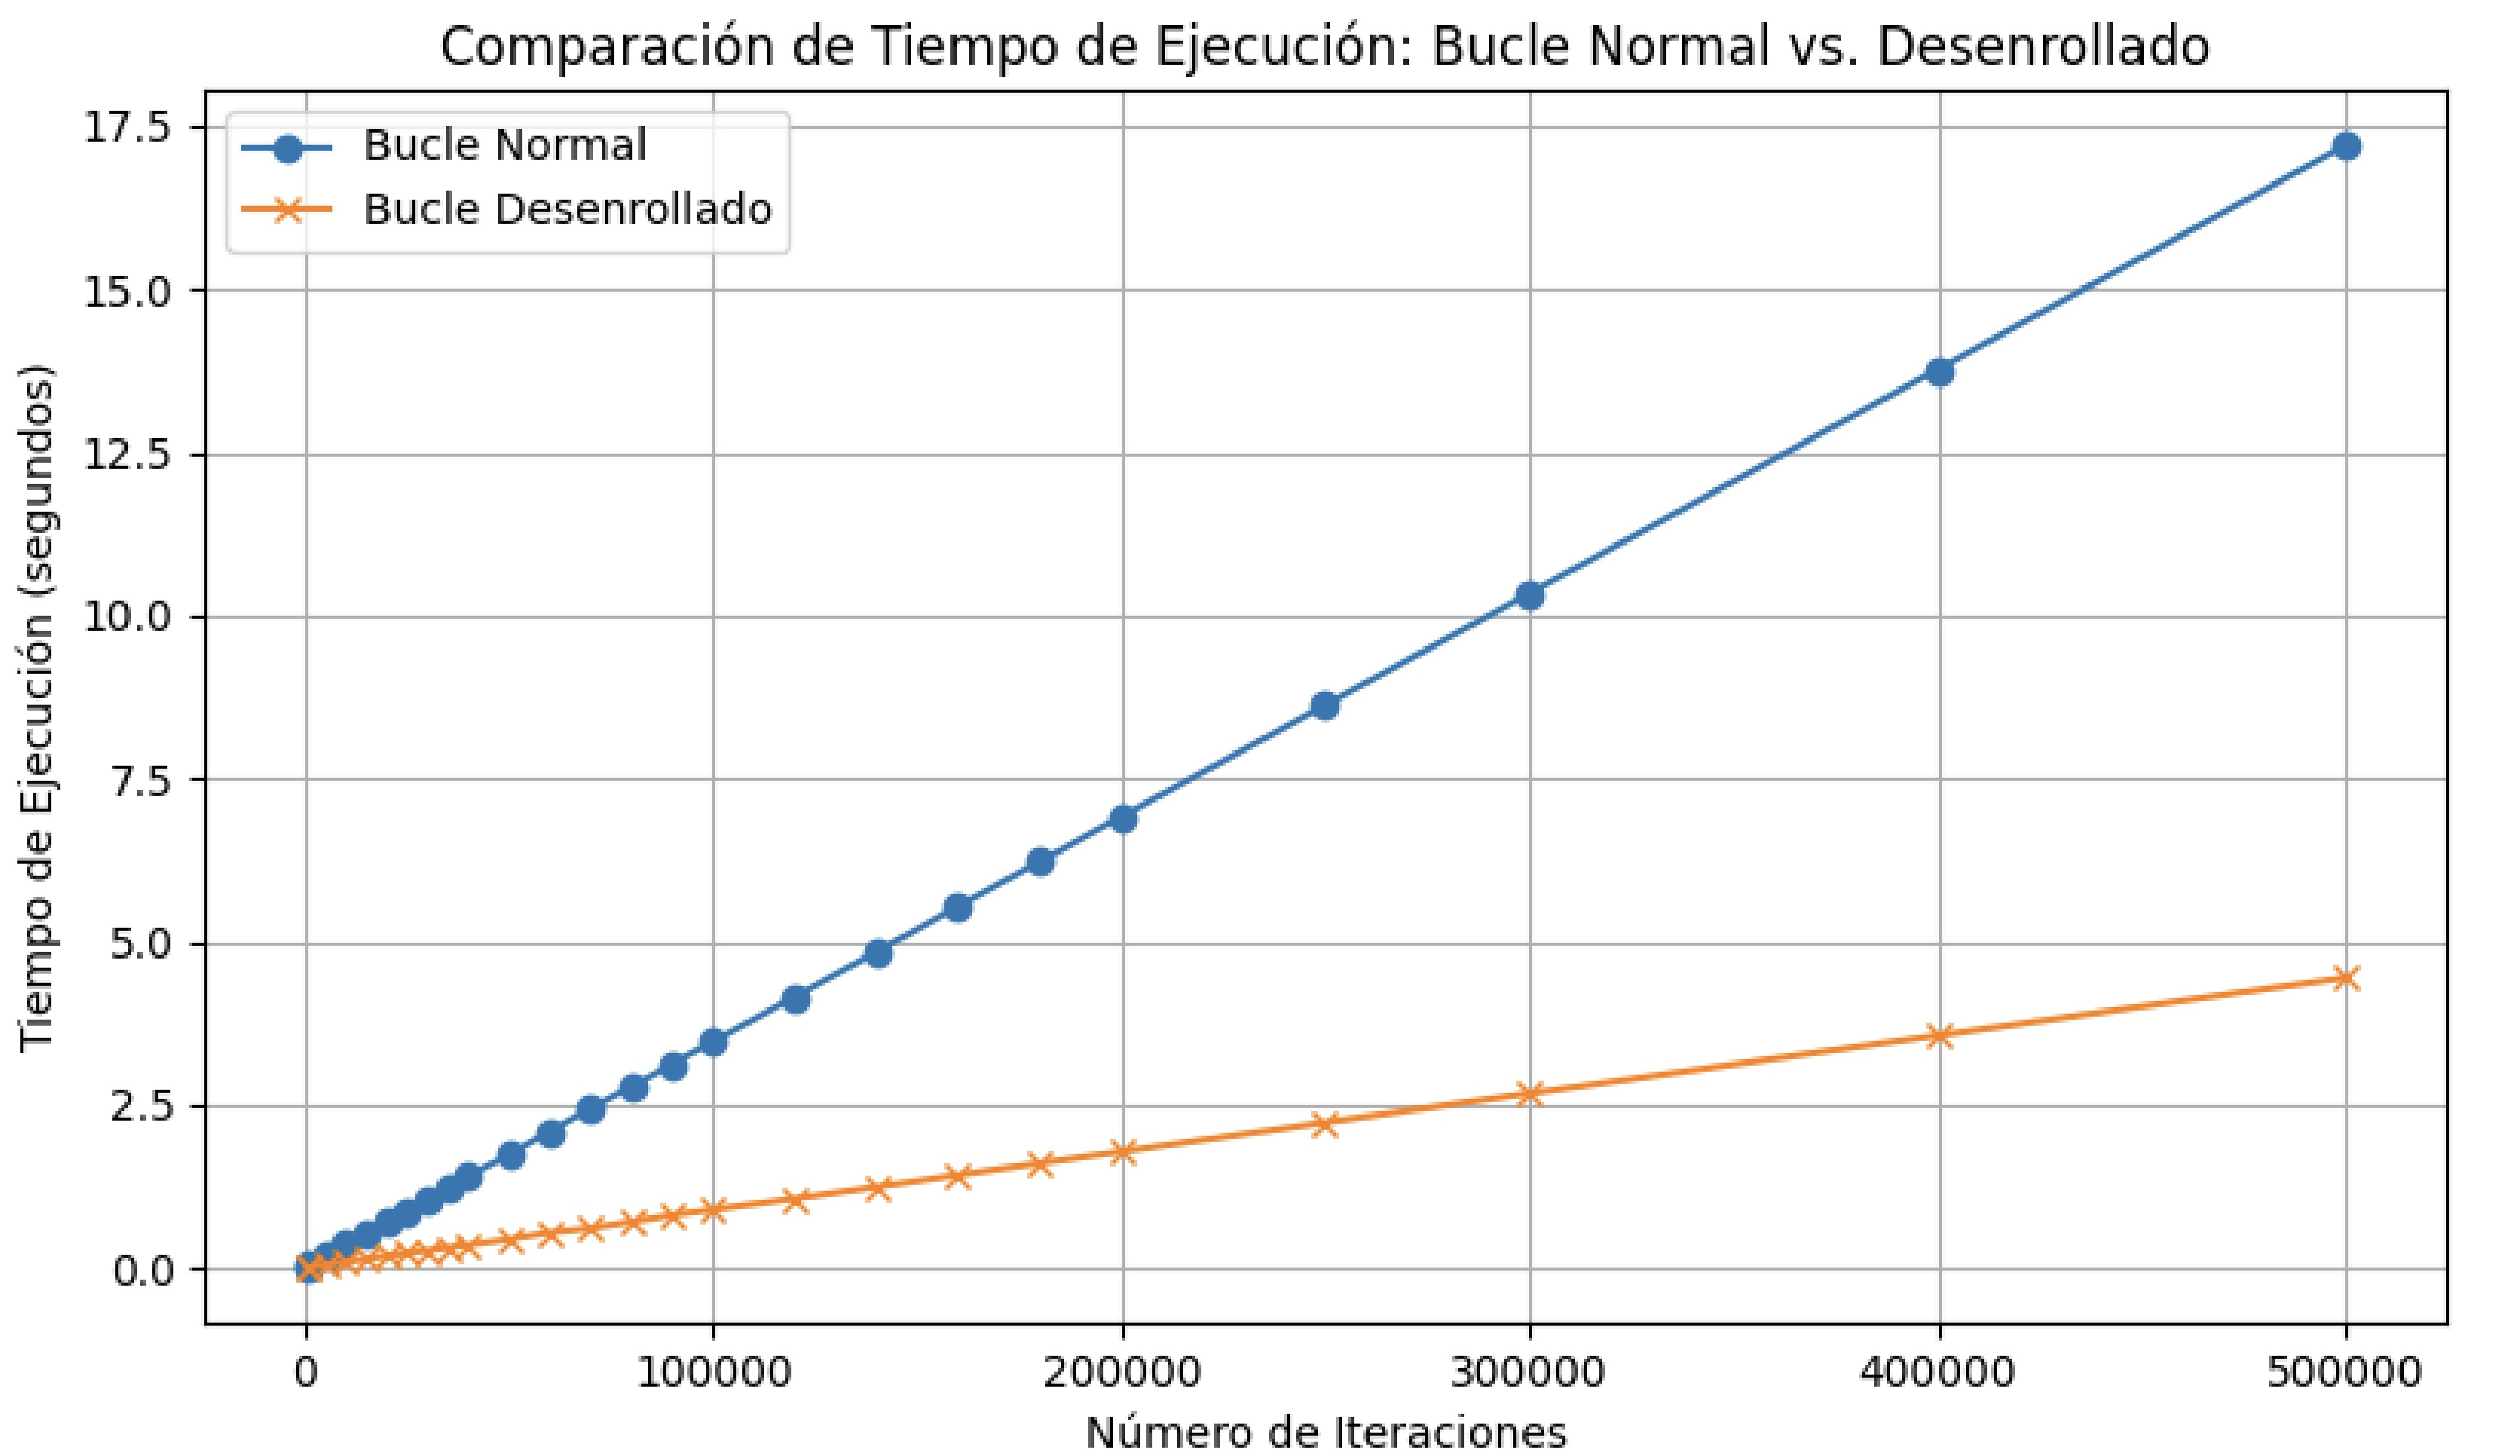
\includegraphics[width=\columnwidth]{img/exeTimes.jpg}
    \caption{Gráfica de tiempo de ejecución en función de ITER}
    \label{fig:iter}
\end{figure}

La gráfica nos muestra dos curvas, azul para el bucle normal y naranja para el bucle desenrollado. Como se puede fácilmente observar obtenemo slas siguientes conclusiones:

\begin{itemize}
    \item \textbf{Mejora del rendimiento con el desenrollamiento:} El bucle desenrollado muestra consistentemente tiempos de ejecución inferiores en comparación con el bucle normal a lo largo de todo el rango de iteraciones. Esto indica que el desenrollamiento de bucles puede ser una técnica efectiva para optimizar el rendimiento de los programas en términos de tiempo de ejecución.
    \item \textbf{Escalabilidad:} A medida que aumenta el número de iteraciones, el impacto del desenrollamiento de bucles en la mejora del rendimiento parece ser más pronunciado. La curva del bucle normal muestra un crecimiento más rápido que la del bucle desenrollado, lo que sugiere que la técnica de desenrollamiento se vuelve más ventajosa a gran escala.
    \item \textbf{Crecimiento lineal:} Ambas curvas parecen seguir un patrón de crecimiento lineal, lo cual es esperable ya que el tiempo de ejecución debería aumentar proporcionalmente con el número de iteraciones. No obstante, la pendiente de la curva del bucle desenrollado es claramente menos inclinada, lo que sugiere una menor adición de tiempo por cada iteración adicional en comparación con el bucle normal.
\end{itemize}

Sin embargo, y a pesar de las mejoras descritas, hay que tener en cuenta que con números bajos de iteraciones, ambos bucles no distan tanto en tiempo de ejecución, por lo que habría que estudiar si en estos casos sería beneficioso aplicar la técnica.

\subsection{Por tamaño de array}

En este segundo experimento a realizar, haremos lo contrario al anterior, es decir, mantendremos un tamaño fijo de iteraciones (5000) y variaremos el tamaño del array.

Esto nos permitirá ver como el unrolling afecta a diferentes tamaños de datos, y si verdaderamente es eficaz, frente a un bucle normal sin desenrollar.

Como en el anteriro experimento nos serviremos de la siguiente gráfica, donde el eje X es el tamaño del array (N) y el eje Y el tiempo de ejecución:


\begin{figure}[H]
    \centering
    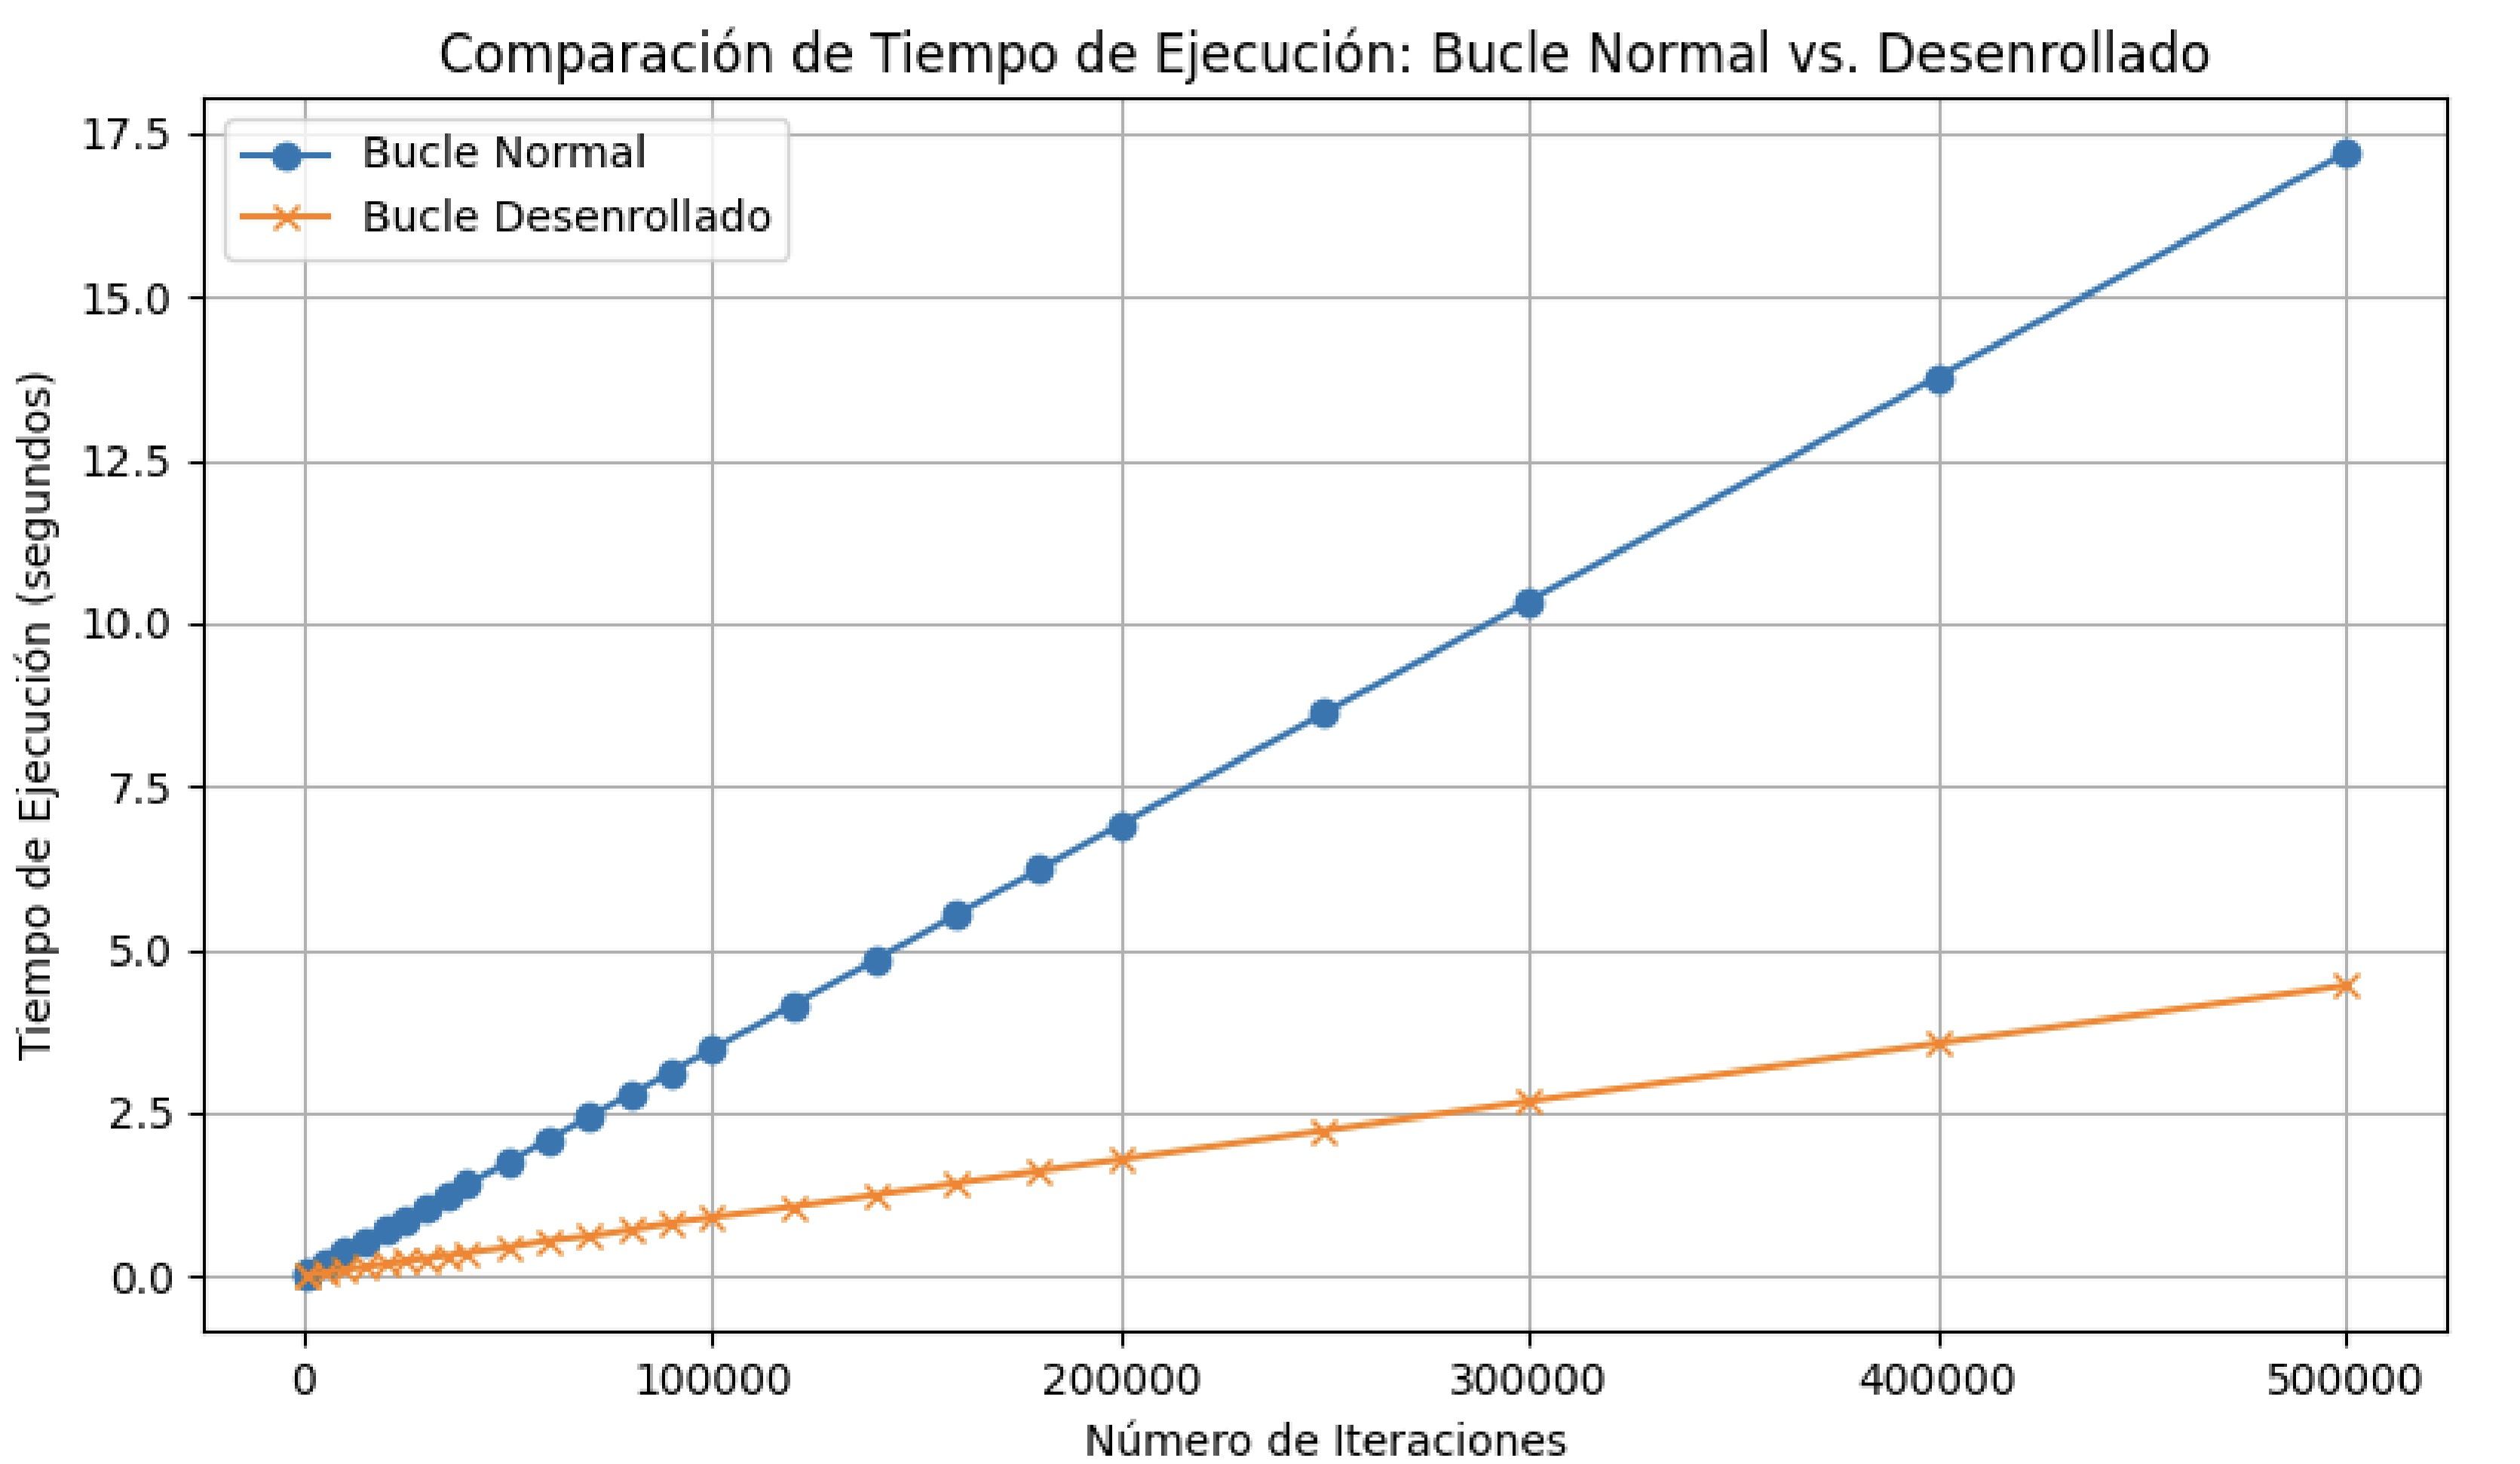
\includegraphics[width=\columnwidth]{img/arrayTam.jpg}
    \caption{Gráfica de tiempo de ejecución en función de N}
    \label{fig:iter}
\end{figure}

Al igual que en el experimento anterior, podemos sacar unas conclusiones similares:

\begin{itemize}
    \item El tiempo de ejecución para el bucle normal aumenta linealmente con el tamaño del array, lo que indica una relación directa entre el tamaño del array y el tiempo de cómputo requerido.
    \item El bucle desenrollado demuestra una eficiencia notablemente mayor. Aunque el tiempo de ejecución también crece con el tamaño del array, lo hace a una tasa menor que el bucle normal.
    \item La diferencia de tiempo entre los dos enfoques se amplía con el aumento del tamaño del array. Esto sugiere que para arrays grandes, el desenrollamiento de bucles puede ser especialmente beneficioso.
    \item La técnica de desenrollamiento de bucles se confirma como una optimización efectiva para la reducción de la sobrecarga de los bucles y el aprovechamiento del paralelismo del hardware, lo cual es crítico en aplicaciones de procesamiento de datos de gran volumen.
\end{itemize}

Estos resultados son muy similares a los obtenidos en el experimento anterior, lo que nos lleva a pensar que la técnica de desenrollamiento de lazos es efectiva en la reducción de tiempos de ejecución en bucles de gran tamaño.

\subsection{Mejora de Rendimiento}

En este apartado vamos a calcular el porcentaje de mejora de rendimiento de una técnica respecto a la otra aplicando la siguiente fórmula:

\begin{equation}
    \text{Mejora de Rendimiento (\%)} = \left( \frac{ts - td}{ts} \right) \times 100\%
\end{equation}

Donde \( ts \) representa el tiempo sin desenrollar y \( td \) el tiempo con desenrollado. 

Para representar esto nos serviremos del siguiente historiograma:   

\begin{figure}[H]
    \centering
    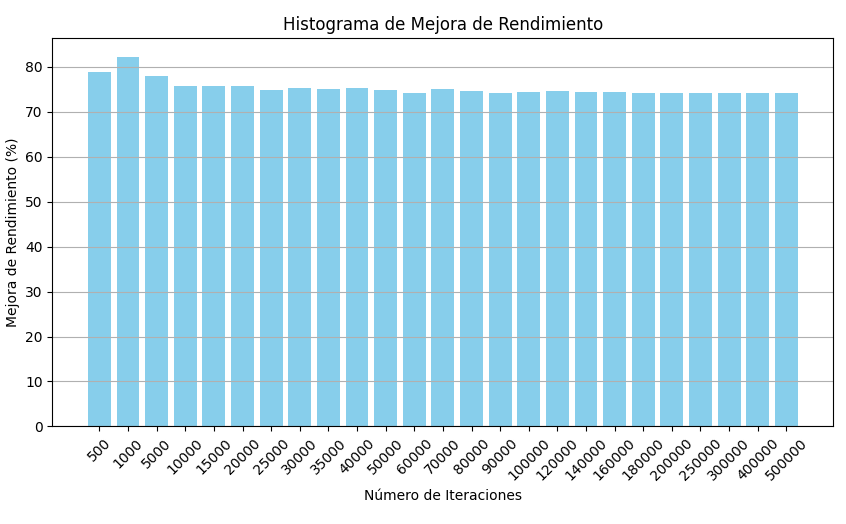
\includegraphics[width=\columnwidth]{img/improvement.png}
    \caption{Histograma de la mejora de rendimiento al aplicar la técnica de desenrollamiento de bucles.}
    \label{fig:histograma_mejora_rendimiento}
\end{figure}


A partir del histograma, se pueden extraer varias conclusiones:

\begin{itemize}
    \item La mejora de rendimiento tras aplicar el desenrollamiento de bucles es consistentemente positiva, lo que indica que esta técnica ofrece beneficios en todos los casos probados.
    \item La mejora porcentual parece ser más significativa en tamaños de array más pequeños. Esto puede deberse a que el desenrollamiento reduce la sobrecarga del control del bucle, que es más notable cuando la carga de trabajo del bucle es menor.
    \item A medida que el tamaño del array aumenta, la mejora porcentual se reduce. Sin embargo, incluso para los tamaños de array más grandes, la técnica aún proporciona un beneficio notable.
\end{itemize}

Es importante considerar que el desenrollamiento de bucles puede introducir complejidad adicional en el código y podría aumentar el tamaño del binario final. Por lo tanto, la decisión de aplicar esta técnica debe balancear la mejora de rendimiento contra estos posibles inconvenientes.

\subsection{Dispersión de Eficiencia de Caché}

Como útlimo experimento vamos a estudiar la eficiencia de caché de ambas técnicas. Para ello, vamos a calcular los "misses" de caché para cada técnica, y veremos como eso afecta al tiempo de ejecución.

En términos de arquitectura de computadoras, los "misses" de caché, también conocidos como fallos de caché, se producen cuando los datos requeridos por la CPU no están disponibles en la memoria caché. En consecuencia, se realiza una operación de acceso a la memoria principal para recuperar estos datos. Este proceso implica una latencia significativamente mayor comparada con la recuperación de datos directamente desde la caché, lo que resulta en un aumento en el tiempo de ejecución del programa.

Para el estudio de lo anterior, utilizaremos la herremienta valgrind, con el siguiente comando:

\begin{lstlisting}[caption={Comando para ejecutar valgrind},label={lst:codigoC}]
    valgrind --tool=cachegrind ./unrolling <array size> <no. of iterations> -O0
\end{lstlisting}

Para el estudio de los resultados, separamos las técnicas en dos códigos diferentes, para poder hacer uso del valgrind de manera correcta. Fijamos el numero de iteraciones en 5000 y aumentamos el tamaño del vector, empezando por 500 y acabando en 100000, dando saltos de 5000 en 5000. 

Una vez ejecutamos el código, obtenemos los siguientes resultados:

\begin{enumerate}
    \item En primer lugar vamos a comparar los misses de caché totales para ambas técnicas:
    \begin{figure}[H]
        \centering
        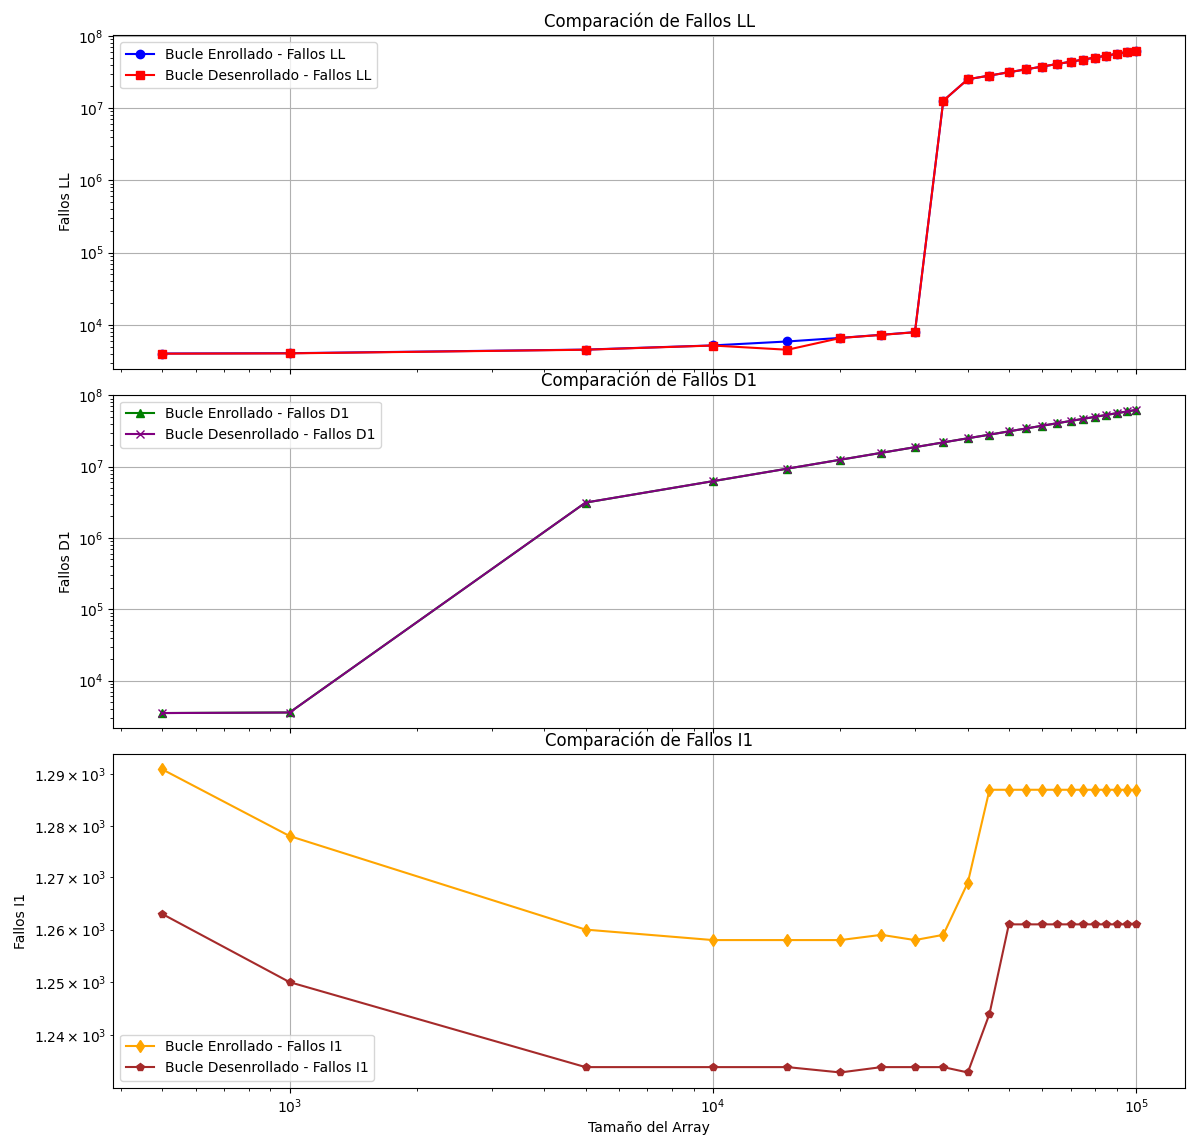
\includegraphics[width=\columnwidth]{img/numberMisses.png}
        \caption{Comparación de misses de caché totales para bucles normal y desenrollado.}
        \label{fig:real_vs_cpu_time}
    \end{figure}
    
    En la imagen podemos observar tres gráficas, que representan los misses de caché para la LL (Last Level), la I (Instrucciones) y la D (Datos). Es destacable que tanto en la LL como en la D1 (Datos de nivel 1) los fallos son similares para ambas ténicas, solo distando en ciertos puntos que puede deberse a una ejecución concreta del programa, es decir, podemos decir que en general para estas dos cachés el número de misses es similar.

    Por otra parte cabe destacar el enorme crecimiento que se procuve en la gráfica de LL que coincide con el tamaño de array de 35 000. Esto puede deberse a que a partir de cierto tamaño entre 30 000 y 35 000, el array supera el tamaño de la caché, lo que provoca un gran aumento de fallos en la caché. 

    En la caché D1, podemos ver que el crecimiento es cuasi-lineal, solo distando de una lineal en los primeros tamaños, que no producen tantos fallos. 

    Por último, en la caché de instrucciones, podemos ver que hay un decrecimiento en el número de fallos, hasta que llega un determinado tamalo de array, donde se produce un salto creciente y despues se mantiene constante. Este saltop tambien coincide con el tamaño de array de 35 000, lo que nos lleva a pensar que a partir de este tamaño, el programa empieza a tener problemas con la caché de instrucciones, y que después a partir de 45 000 se mantiene constante, lo que puede deberse a que accede a todas las intrucciones únicas necesarias para el programa y las guarda en la caché.

    Esta última es la única gráfica donde podemos ver que el bucle desenrollado tiene menos fallos que el bucle normal (lo que se debe a que accede a menos instrucciones), lo que nos lleva a pensar que el desenrollamiento de lazos puede ser beneficioso en este aspecto.

    \item Por otra parte vamos a realizar las mismas gráficas pero ahora haciendo el ratio fallo por acceso, para ver como afecta el desenrollamiento de lazos a este ratio:

    \begin{figure}[H]
        \centering
        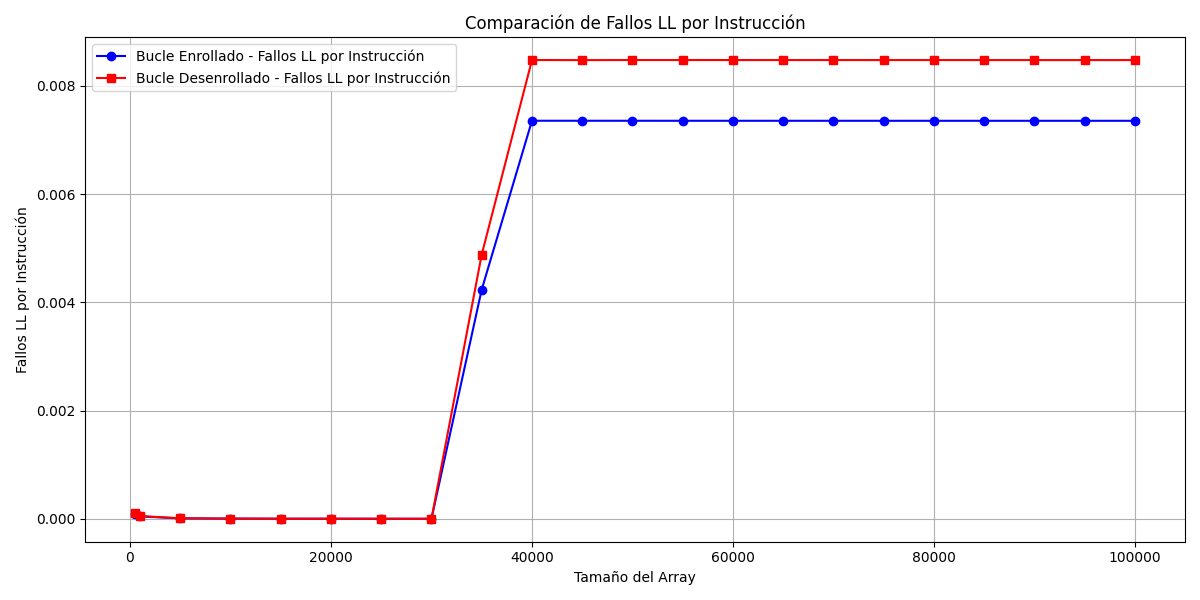
\includegraphics[width=\columnwidth]{img/Fallos_LL.png}
        \label{fig:real_vs_cpu_time}
    \end{figure}

    \begin{figure}[H]
        \centering
        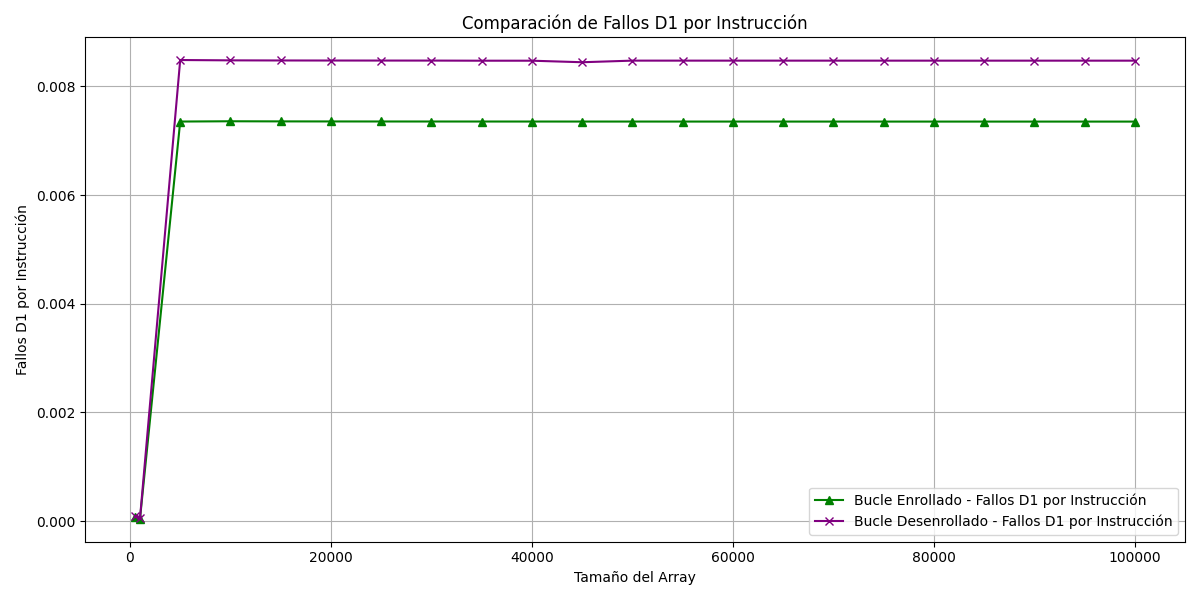
\includegraphics[width=\columnwidth]{img/Fallos_D1.png}
        \label{fig:real_vs_cpu_time}
    \end{figure}

    \begin{figure}[H]
        \centering
        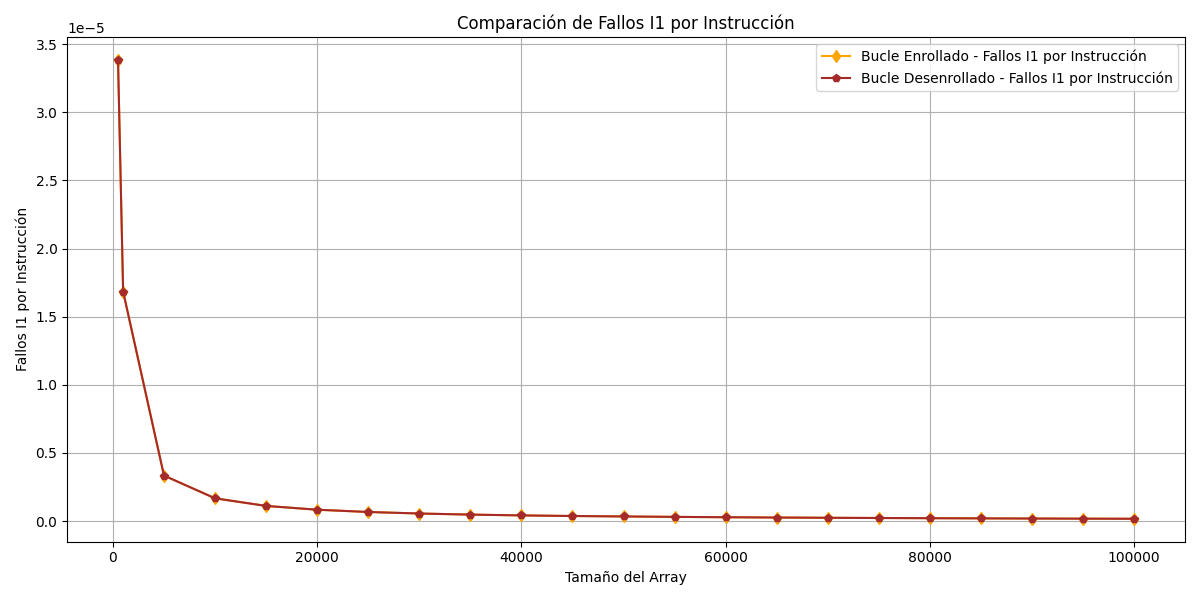
\includegraphics[width=\columnwidth]{img/cacheRatioI1.png}
        \caption{Comparación de ratio de misses de caché para bucles normal y desenrollado.}
        \label{fig:real_vs_cpu_time}
    \end{figure}

    Para mejorar la visualización, ponemos la gráfica sin escalas logarítmicas, ya que al ser un ratio, no es necesario. 

    Si nos fijamos tanto en las gráfica de la caché LL como la de la D1, podemos ver un resultado que se diferencia de las conclusiones del anterior punto. Esto es, a pesar de que en fallos totales es mejor el bucle desenrollado, al hacer el ratio podemos ver que el bucle normal tiene menos fallos por acceso que el desenrollado. Esto se puede deber a que al desenrollar el bucle se accede a más datos en memoria por iteración, lo que puede aumentar la presión sobre la caché de datos, provocando un aumento general en el número de fallos por acceso.

    Por otra parte, podemos ver que a su vez el ratio para la caché de instrucciones es el mismo, y que es completamente decreciente por número de accesos.
\end{enumerate}

Con los resultados anteriores podemos concluir que en términos de eficiencia caché, a pesar de que el bucle desenrollado tiene menos fallos totales, el ratio de fallos por accesos es mayor, por lo que habría que considerarlo a la hora de aplicar la técnica.

\section{Análisis del código ensamblador}

Para finalizar, estudiamos el código ensamblador generado con la herramienta \href{https://godbolt.org/}{Godbolt}, para ver poder comparar el código generado por ambas técnicas.

Como podemos comprobar al meter el código en la herramienta el código generado por el bucle desenrollado es mucho más largo que el generado por el bucle normal, lo que puede llevar a pensar que el desenrollamiento de lazos puede ser beneficioso en términos de tiempo de ejecución, pero perjudicial en términos de tamaño del binario final. 

Por tanto, al ser el código generado más largo, la eficiencia espacial del código se ve reducida al introducir el desenrollamiento de bucles, lo que puede ser un factor a tener en cuenta a la hora de aplicar la técnica.

%------------------------------------------------
	
\section{Conclusiones}

Podemos concluir que una vez realizados los experimentos, el desenrollamiento de lazos es una técnica efectiva para la optimización de bucles en términos de tiempo de ejecución, pero tenemos que tener en cuenta que aumenta el tamaño del binario final y puede reducir la eficiencia espacial. 

A pesar de todo esto, el "unrolling" resulta en la mayoría de casos una herramienta efectiva, y puede ayudar a reducir el tiempo de ejecución de los programas en bucles con un gran número de datos.

%----------------------------------------------------------------------------------------
%	Referencias
%----------------------------------------------------------------------------------------
	
\begin{thebibliography}{99} % Bibliografía - alternativamente, se recomienda el uso de bibtex o biblatex

    \bibitem[1]{LoopUnrollingGeeksforGeeks}
    GeeksforGeeks.
    \newblock {\em Loop Unrolling}.
    \newblock \url{https://www.geeksforgeeks.org/loop-unrolling/}, \newblock [online]
    
    \bibitem[2]{Dragomir2009}
    O. S. Dragomir, T. Stefanov, and K. Bertels.
    \newblock Optimal Loop Unrolling and Shifting for Reconfigurable Architectures.
    \newblock {\em ACM Transactions on Reconfigurable Technology and Systems}, Vol. 2, No. 4, Article 25, September 2009, 24 pages.
    \newblock DOI = 10.1145/1575779.1575785.
    \newblock \url{http://doi.acm.org/10.1145/1575779.1575785}, \newblock [online]

    \bibitem[3]{Buyukkurt2004}
    Betul Buyukkurt, Zhi Guo, and Walid A. Najjar.
    \newblock {\em Impact of Loop Unrolling on Area, Throughput and Clock Frequency in ROCCC: C to VHDL Compiler for FPGAs}.
    \newblock Department of Computer Science and Engineering, University of California - Riverside, Riverside, CA 92507, USA.
    
\end{thebibliography}


	
	%----------------------------------------------------------------------------------------
	
\end{document}

